% Created 2023-03-27 Mon 15:28
% Intended LaTeX compiler: pdflatex
\documentclass[11pt,congress]{ieeetran}
\usepackage[utf8]{inputenc}
\usepackage[T1]{fontenc}
\usepackage{graphicx}
\usepackage{longtable}
\usepackage{wrapfig}
\usepackage{rotating}
\usepackage[normalem]{ulem}
\usepackage{amsmath}
\usepackage{amssymb}
\usepackage{capt-of}
\usepackage{hyperref}
\usepackage{numprint}
\author{Sergi Simón Balcells}
\date{\today}
\title{Window approach to a forum encryption system}
\hypersetup{
 pdfauthor={Sergi Simón Balcells},
 pdftitle={Window approach to a forum encryption system},
 pdfkeywords={},
 pdfsubject={},
 pdfcreator={Emacs 28.2 (Org mode 9.6.1)}, 
 pdflang={English}}
\begin{document}

\maketitle
\begin{abstract}
An online forum is a platform that enables users to post messages which become available to any
person with access to it. In this article, we focus on forums that preserve the anonymity of a
user while being authenticated. More concretely, in this paper, we improve an existing scheme.
\\\\
Index terms - cryptography, discussion board, privacy, ring signature
\end{abstract}

\section{Introduction}
\label{sec:orgba5403b}
Enterprises, city halls, and educators found a way to guarantee anonymous feedback by providing a mailbox
where people could post a message without specifying who it was. This enabled workers, citizens, and students
to provide feedback without any chance of having repercussions for criticizing them. At the same time, as the location of them was inside of the enterprise, city, and educational center, the readers could assert with some
security that the writer was, in fact, an employee, a citizen, and a student.

With the arrival of the Internet, some of these activities could be online, as a remote
office, so it made apparent that there is a need for a security protocol that preserves the
anonymity of the poster while it makes sure that the writer is an authenticated user. This use case
will be referred to as a forum in this paper.

Such a cryptographic system should provide a means to authenticate, so only users can post messages. The users
should remain anonymous, as the identity of the message author is not revealed. Additionally, messages from the same user should remain unlinkable.

For this cryptographic scheme, a Group signature \cite{group} could provide the required security purposes. However, this cryptographic scheme includes a trusted group manager, who can revoke the anonymity of the writer when required. To overcome this difficulty, the protocol described here will use a similar tool, namely, ring signatures \cite{ring}. This does not require its users to trust the entity except for
certificate authorities issuing public key certificates.

\section{Preliminaries}
\label{sec:orgc6e8a58}
Before continuing, a few concepts have to be made clear to explain the algorithm and the caveats of the
previous work. Concretely, both group and ring signatures have to be explained, as well as the distribution that the Internet posters follow.

\subsection{Group Signature}
\label{sec:org8b94944}
Group signatures \cite{group} are a cryptographic protocol that lets a user sign as a group of users. The
use case for this protocol is enterprises or city halls, where one worker could make an official statement
without needing a centralized user for everyone or specifying who in the group has signed. This is a better
approach to publishing an official statement, as this needs a centralized user, which attacks through social engineering, such as fishing, could make more damage than a non-centralized user. Nevertheless, it needs a trusted middleman to encrypt securely the message, and this middleman knows who has posted the message. For this specific reason, this protocol can not be used in our public encryption, as the sole purpose of signing the message is to make sure that the centralized forum \textbf{does not know} who has posted it.

\subsection{Ring Signature}
\label{sec:orgd2e2b3b}
On the other hand, ring signatures \cite{ring} provides the same as group signatures without the middleman, and as such is the perfect cryptographic protocol to base the forum cryptographic system. The idea is that every message is signed by a subgroup of the forum users, such as 8 users. This provides anonymity of the user of \(\frac{1}{8}\) chances of being the real original poster. Additionally, efficient ring signatures exist \cite{ring-rsa}, where the size of the public key does not depend on the size of the group signature, making it painless to improve security by providing a larger public key for encryption.

Then, the problem for this algorithm is choosing the users that should fill the space of signatures. In the next subsection, we will discuss which distribution the internet posts follow.
\subsection{Internet post distribution}
\label{sec:orgdc5dcbb}
The reality between the distribution of the messages and the posters makes such a random
assignment impossible to hold. Posters have an empirically 90-9-1 percent approach to posting, where the 90\%
of the users barely post (lurkers), 1\% of the users post most of the content (superusers), and 9\% percent of
the users post more regularly but not as outlying as the 1\% (users). The \cite{zipf} article analyzes this
distribution, where it explains that the known Zipf law adapts well to simulate this posting scenario.

Using a randomly assigned group and knowing that the distribution follows the Zipf law, makes the superusers
anonymous, that is, the number of signatures that a user appears divided by the number of messages posted, close to one, which in turn means that the most of its signatures are also their posts. This makes it not secure to use a randomly assigned group approach for signing in to an online forum.



\section{Caveats of previous approach}
\label{sec:org2816147}
The previous algorithm \cite{recsi} queried all the previous messages that have been sent in the forum and attaches a weight depending on the number of messages. The thought is that the algorithm will adapt to those users that have a large number of signatures as superusers and give them more weight, those solving the problem that a random approach had. The problem is the initial number of messages, as most weights sky-rocket the number of signatures so that the anonymity in the super users is astonishingly high on average but close to non-existence for lurkers that started sending messages later on. The solution was to increase the initial message weight so that the weight added for signatures didn't matter as much, but the sheer amount of signatures on the superuser would still provide better anonymity for them.

This solution was inconvenient because it sacrificed the anonymity of both lurkers and superusers. It was discussed that a time weight, that is, the weight of a signature is decreased with time.

Another problem is the lack of scalability. As more messages are posted in the forum, more costly is to send another message, as you have to add all the weights to be able to sign. This is not a problem with smaller forums, but consider that this forum is used in a big city with millions of habitants. It could potentially mean that after some years, it is not possible to post anymore. For this reason,  instead of decreasing the weight with time, creating a window of the last \(n\) signatures and computing the weight with them, would be more efficient. Additionally, as the window is limited, there is a limit on the weight the user can carry, possibly making the algorithm solve the snowballing effect.

Finally, although most user-centered content behaves in the 90-9-1 scheme, we are not sure if this pattern would persist if there is a change in the users. Let's say that in an enterprise forum, one of the employees moves to another company. That would change the user posting details, as it would inevitably become inactive. A window approach would treat it naturally, while a preferential attachment would value this user more than a new employee's user.

In conclusion, we think that a time-based window could result in better privacy for the users than the preferential approach previously discussed, as the system will adapt more carefully to the change in user behaviors while solving the snow-balling effect in the preferential attachment system.

\section{Methodology}
\label{sec:org98acfc0}
The anonymity of a user is declared as the number of messages sent divided by the number of messages signed. This will be the most important value that we can use to assert how strong is the cryptosystem. But, let's showcase that it is not valuable for a specific user. If one user has low anonymity, but, with the same number of signatures, most users have high anonymity, then it's impossible to discern which is the low anonymity user, as the attacker would a priori only have the signatures as a way to tell which user posted. As such, it matters the average or the median of anonymity in a group of users with a similar number of signatures.

Now, in a simulation, we can find the distribution of signatures. Although the messages rarely receive a Zipf distribution, the final distribution of signatures should be more normalized. A quick execution \ref{fig:sign-dist} showcases that the number of signatures peaks at 80 signatures, and it has a more defined normal distribution. For this reason, to describe groups with a similar number of signatures we used quantiles of the users, which would provide a more meaningful insight that all of them grouped.

\begin{figure}[htbp]
\centering
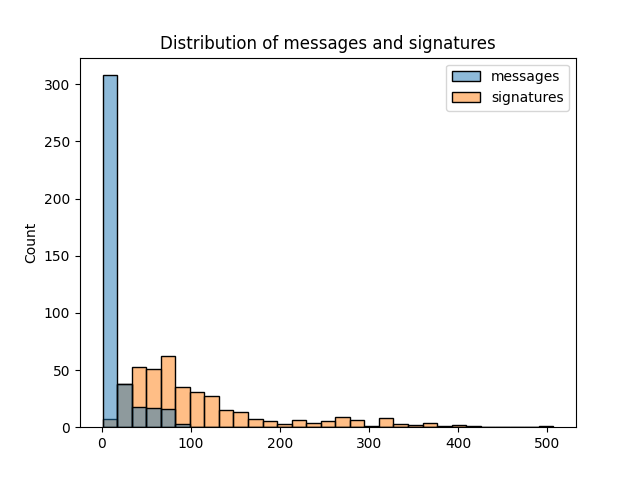
\includegraphics[width=.9\linewidth]{sign-dist.png}
\caption{\label{fig:sign-dist}Distribution of messages and signatures. As seen, most users only post one message, while they appear on 80 signatures.}
\end{figure}

Additionally, it was regarded as necessary to test how much anonymity has a message that hadn't appeared in the window before. As messages outside of the window don't have the same probabilities to appear, this could mean that they only appear on the window when they post, which would mean that they don't have as much anonymity.

With all this information, a simulation program has been made. It can be seen in \href{https://github.com/sergisi/glowing-dollop}{this link}. The simulation creates a Zipf distribution, runs a simulation for the encryption method, and either provides the statistical analysis by itself or leverages a CSV, where each row represents a user with the number of messages posted and the number of signatures posted.


\section{Results}
\label{sec:org715c89b}
The results can be shown in \ref{tab:results}. First, the parameters of the preferential attachment are provided to prevent bad lurkers, which means that the initial weight that all users have is 5 times higher than the message weight. Second, the most important metric is comparing the lowest score of the same group. In this example, super-users have the lowest score in total messages on the preferential signature, which makes it the worst-case scenario in this example. The first column means the type of reviewer that it has, where the first item in a group represents the analysis, and the subsequential groups represent those in the quartiles that define lurkers, users, and super-users. The parameters of the simulation are as follows: 400 people, 8 people per signature, 100 messages for the most active user 20 messages for the window. Window signature has 1 of initial weight and 20 for each message that appears in the window. The preferential signature has an initial weight of 5 and adds 1 for each signature. Lurkers are defined as the first 0.01 quantile and superusers as the last 0.01. The parameter \(s\) of the Zipf distribution is 1.2.

\begin{table}[htbp]
\caption{\label{tab:results}Results of the simulation.}
\centering
\begin{tabular}{lrr}
Reviewer & Mean & Median\\[0pt]
\hline
first-message & 6.801 & 5.5\\[0pt]
lurkers & 5.5 & 6.0\\[0pt]
users & 6.815 & 5.5\\[0pt]
superusers & 6.776 & 5.778\\[0pt]
\hline
window & 27.464 & 14.833\\[0pt]
lurkers & 13.375 & 17.0\\[0pt]
users & 27.836 & 15.0\\[0pt]
superusers & 5.139 & 5.193\\[0pt]
\hline
preferential & 33.118 & 18.0\\[0pt]
lurkers & 14.542 & 21.0\\[0pt]
users & 33.599 & 18.0\\[0pt]
superusers & 4.581 & 4.630\\[0pt]
\end{tabular}
\end{table}

A quick distribution plot can be shown that even if there are some users with bad privacy, they are practically invisible as their peers have strong privacy. Figure \ref{fig:swarm-anonlog} shows that even those with low anonymity are surrounded by users with strong anonymity the lurkers and normal users, while the superuser has more consistent anonymity.

\begin{figure}[htbp]
\centering
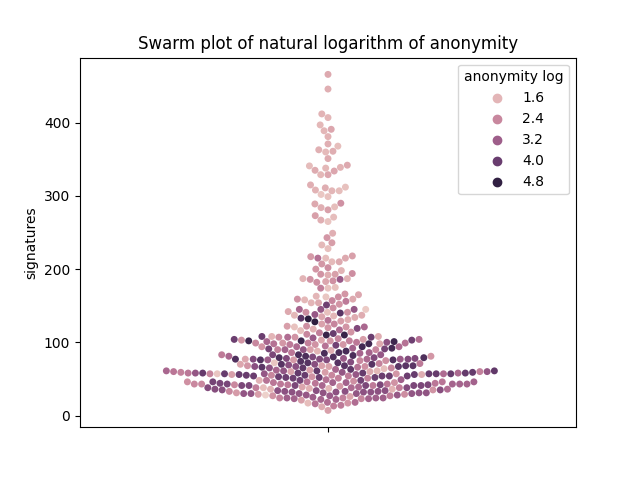
\includegraphics[width=.9\linewidth]{anonlog-swarm.png}
\caption{\label{fig:swarm-anonlog}Swarm plot of the different figures. Due to several outliers with strong anonymity, it is shown as the natural logarithm of anonymity rather than itself. It showcases that most of the super-users have a better score, while the normal users that have the lowest are camouflaged by lurkers that have the largest amount of anonymity.}
\end{figure}

\section{Conclusions}
\label{sec:org7b5276e}
The simulation of both algorithms has provided some insight into the parameters that work well between these two. The preferential attachment works surprisingly well if a high score is given initially, but it distributes less equally the anonymity between the different groups of users. On the other hand, the window approach it's not as constrained by the initial parameters, and overall offers better anonymity than the preferential attachment.

Nevertheless, as stated before, the window approach should be better for scaling the forum, as it does not need to receive all the messages to compute the group encryption while being more restraint against the snowballing effect previously noticed in the preferential attachment.

As such, it is concluded that the window approach is an improvement of the existing algorithm.

\section{Acknowledgements}
\label{sec:orge635b51}
This project follows the discussions that were done in the RECSI cryptographic congress, where a time-based approach was discussed if it could solve the snowballing effect on the preferential system. As such, this project would have not been made if we were not invited to the RECSI congress.

\bibliography{bib}
\bibliographystyle{ieeetr}
\end{document}